\documentclass[tikz,border=8pt]{standalone}
% Shared look for every TikZ diagram. Load with \input{../../tools/tikz-style.tex}
\usepackage[T1]{fontenc}
\usepackage{lmodern}
\renewcommand{\sfdefault}{lmr}  % diagrams use the same serif as the text
\usetikzlibrary{arrows.meta, positioning, shapes.geometric, calc, fit, backgrounds}
\definecolor{cblue}{HTML}{4C78A8}
\definecolor{corange}{HTML}{F58518}
\definecolor{cgreen}{HTML}{54A24B}
\definecolor{cred}{HTML}{E45756}
\definecolor{cpurple}{HTML}{B279A2}
\definecolor{cgrey}{HTML}{6B6B6B}
\tikzset{
  every picture/.style={font=\sffamily, line width=1.2pt},
  box/.style={draw=#1, fill=#1!12, rounded corners=4pt, align=center, inner sep=7pt, minimum height=1.1cm},
  box/.default=cgrey,
  arrow/.style={-{Stealth[length=3mm]}, draw=cgrey, line width=1.4pt},
  title/.style={font=\sffamily\bfseries\Large},
  note/.style={font=\sffamily\small, text=cgrey, align=center},
}
\AtBeginDocument{\hyphenpenalty=10000 \exhyphenpenalty=10000}

% Set-valued (nondeterministic) information state with a sensor that never errs and a move of 1, 2 or 3 cells.
% Row 1: the reading "door" leaves {1, 3, 7}. Row 2: moving 2 (really 1, 2 or 3 cells) gives the union {2,3,4} u {4,5,6}
% u {8,9,0}. Row 3: the reading "door" again keeps only the cells of row 2 that are doors: {3}.
\definecolor{cbrown}{HTML}{9C755F}
\begin{document}
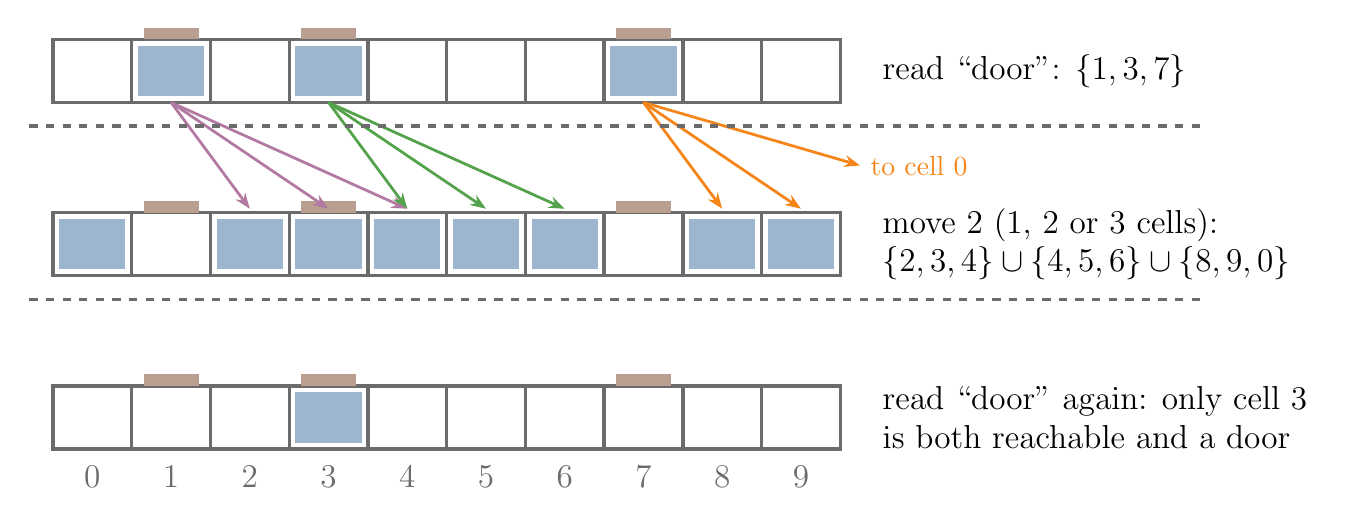
\begin{tikzpicture}[x=1cm, y=1cm, every node/.append style={font=\large}]
  \newcommand{\hall}[3]{% y, list of cells in the set, label
    \foreach \i in {0,...,9} {\draw[cgrey] (\i,#1) rectangle (\i+1,#1+0.8);}
    \foreach \d in {1,3,7} {\fill[cbrown!70] (\d+0.15,#1+0.8) rectangle (\d+0.85,#1+0.95);}
    \foreach \i in {#2} {\fill[cblue!55] (\i+0.08,#1+0.08) rectangle (\i+0.92,#1+0.72);}
    \node[anchor=west, align=left] at (10.4,#1+0.4) {#3};
  }
  \hall{4.4}{1,3,7}{read ``door'': $\lbrace 1, 3, 7\rbrace$}
  \hall{2.2}{0,2,3,4,5,6,8,9}{move 2 (1, 2 or 3 cells):\\$\lbrace 2,3,4\rbrace \cup \lbrace 4,5,6\rbrace \cup \lbrace 8,9,0\rbrace$}
  \hall{0}{3}{read ``door'' again: only cell 3\\is both reachable and a door}
  \foreach \i in {0,...,9} {\node[cgrey] at (\i+0.5,-0.35) {\i};}
  % arrows from each door cell to the cells it can reach (1, 2 or 3 cells to the right)
  \foreach \s/\c in {1/cpurple, 3/cgreen, 7/corange} {
    \foreach \k in {1,2,3} {
      \pgfmathtruncatemacro{\tgt}{\s+\k}
      \ifnum\tgt<10
        \draw[-{Stealth[length=2mm]}, \c, line width=1pt] (\s+0.5,4.4) -- (\tgt+0.5,3.05);
      \fi
    }
  }
  \draw[-{Stealth[length=2mm]}, corange, line width=1pt] (7.5,4.4) -- (10.25,3.6) node[right, font=\normalsize] {to cell 0};
  \draw[cgrey, dashed] (-0.3,1.9) -- (14.6,1.9);
  \draw[cgrey, dashed] (-0.3,4.1) -- (14.6,4.1);
\end{tikzpicture}
\end{document}
